\section{Compiler}

    \subsection{Compiler vs. Intrepreter}
    \begin{frame}[t]{Compiler}\framesubtitle{Compiler vs. Intrepreter}
        \begin{itemize}
            \item Performance
            \item Development Cycle
            \item Debugging
            \item Specific Constraints
        \end{itemize}
    \end{frame}

    \subsection{Compiler Overview}
    \begin{frame}[t]{Compiler}\framesubtitle{Compiler Overview}
        \begin{columns}[t]
            \begin{column}{.48\textwidth}
                \begin{itemize}
                    \item ANTLRv4
                    \item Visitor Pattern
                    \item JAVA
                \end{itemize}
        \begin{figure}[ht]
        \centering
        \resizebox{.9\textwidth}{!}{
        \begin{tikzpicture}
            \matrix (m) [ampersand replacement=\&,matrix of nodes]
            {
             GAMBL  \& $\to$ \&  OpenCL C  \\
                \&  Java    \& OpenCL C \& $\to$ \& \hspace{1 em} M \hspace{2 em}  \\
                \&       \&   \& C  \&         \\
                \&       \&               \\
              };
            \draw (m-1-1.south west) |- (m-1-3.north east) |- (m-2-2.north east) |- (m-2-2.south west) |- (m-1-1.south west);
            \draw (m-2-2.south east) |- (m-2-5.north east) --(m-2-5.south east) -- (m-2-5.south west) |- (m-3-4.south west) |- (m-2-2.south east);
        \end{tikzpicture}
        }
        \end{figure}

            \end{column}
            \begin{column}{.48\textwidth}
                \vspace{-30pt}
                \begin{figure}
                    \centering
                    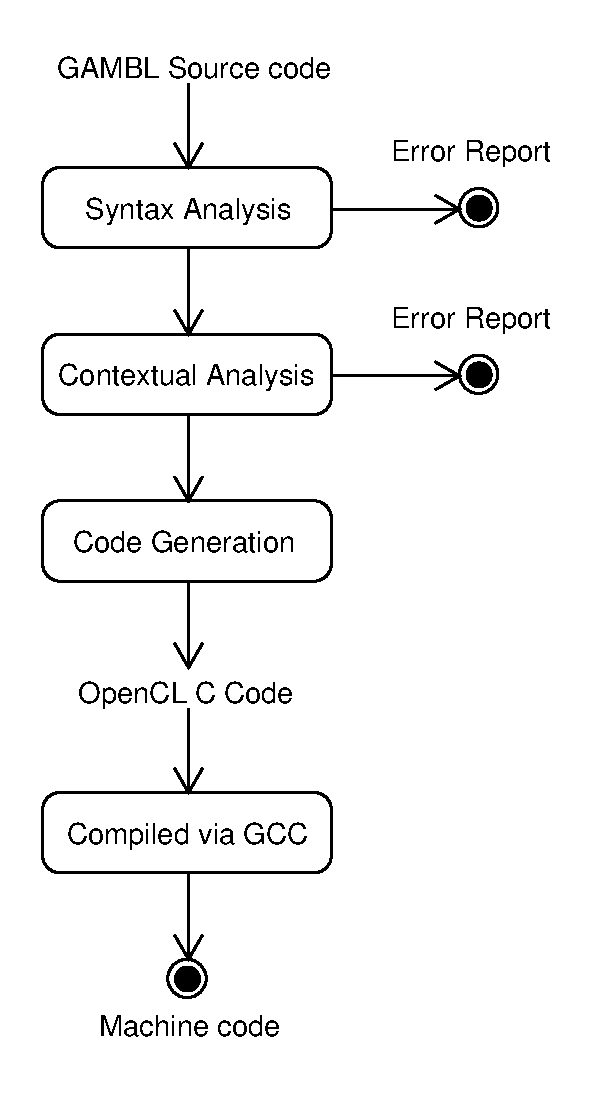
\includegraphics[width=0.8\textwidth]{images/CompilerDiagram.pdf}
                \end{figure}
            \end{column}
        \end{columns}
    \end{frame}

    \subsection{Syntax Analysis}
    \begin{frame}[t]{Compiler}\framesubtitle{Syntax Analysis}
        ANTLR ... ?
    \end{frame}
